\chapter{Implementation}
    Let's prepare the application which will be used all principles describes in~\ref{analysis}. Created project is focused on the design and development of the Automatic prediction model builder system in the form of an application with a user-friendly user interface, which will be implemented in the cloud environment. As a development environment Matlab ecosystem was used.
    \section{Mathematical models}
    Prediction models were based mainly on the principle of linear prediction (LP) and its modifications, such as non-integer linear prediction (fractional linear prediction - FLP), LP extended by parameters capable of capturing short-term and long-term trendiness in data (extended linear prediction - ELP), etc., which will be extended by further statistical methods such as Monte Carlo, Markov chains, etc.\\
    \\
    For the identification of the appropriate structure of economic and behavioral models and the identification of the parameters of the selected models, machine learning algorithms will be used, which will provide the optimal solution for the selected data and thus the use-case.
    \section{Application}
    This application would make it possible to easily and accurately predict various socioeconomic macro and micro indicators, such as gross/net domestic/national product, economic wealth, unemployment, inflation, average/minimum wage, purchasing power of the population but also the behavior of customers (customers can also be perceived as households), intended for sectors such as public or state administration, public planning (but also private) finance, banking.\\
    \\
    From the point of view of commercial use, a possible application would be predicting the number of customers and the number of orders, the company's income, the success of marketing strategies, or on the basis of the prediction, the planning of warehouse stocks.
    \begin{figure}
        \centering
        \begin{subfigure}[b]{0.6\textwidth}
            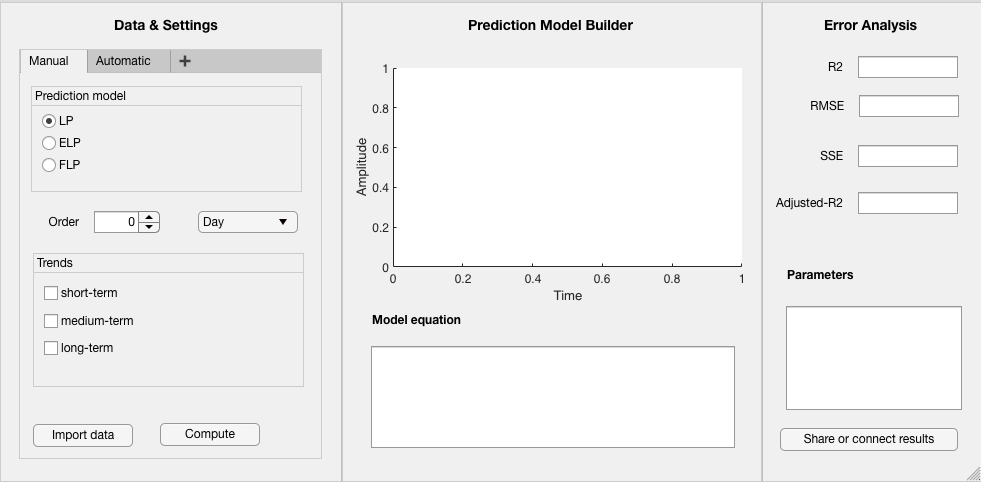
\includegraphics[width=\textwidth]{figures/manual.png}
            \caption{Manual setting}
            \label{fig:manual}
        \end{subfigure}
        \hspace{0.1\textwidth}
        \begin{subfigure}[b]{0.6\textwidth}
            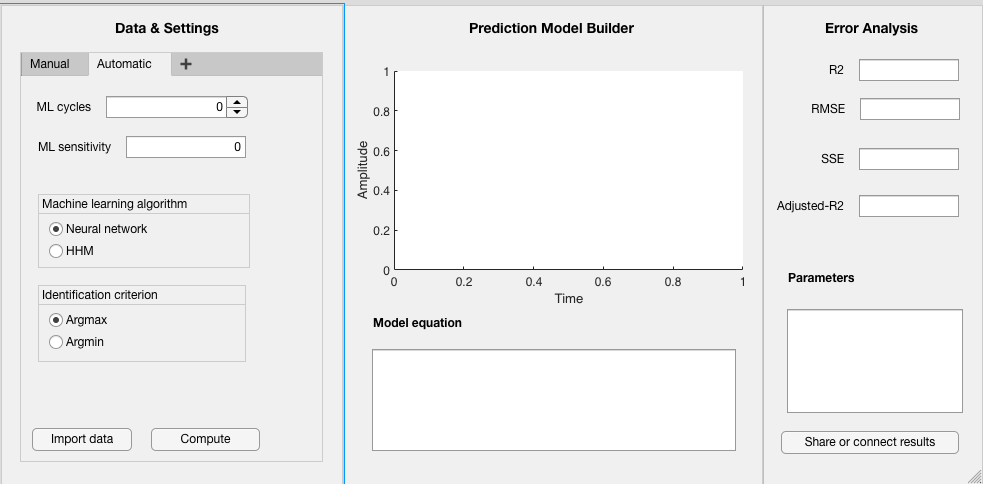
\includegraphics[width=\textwidth]{figures/auto.png}
            \caption{Automatic setting}
            \label{fig:automatic}
        \end{subfigure}
        \begin{subfigure}[b]{0.6\textwidth}
            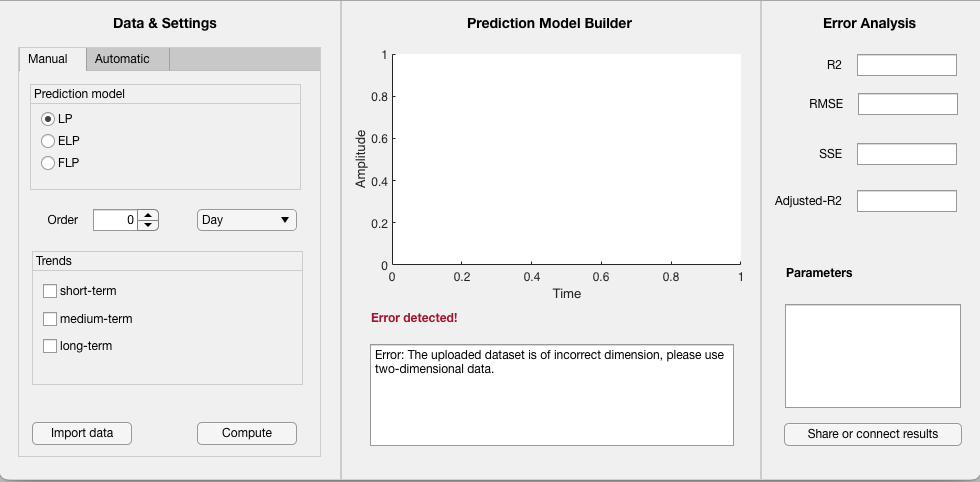
\includegraphics[width=\textwidth]{figures/warning.png}
            \caption{Dataset warning}
            \label{fig:warning}
        \end{subfigure}
        \label{fig:appoverview}
        \caption{Application overview}
    \end{figure}
        \subsection{Import datasets}
        First step to get results from predictive application. Use the button in the left bottom corner~\ref{fig:manual} to import our dataset. Application is able to process datasets in csv or excel format. Application is trying to identify your dataset by the setting~\ref{subsec:setting}. If the problem in our imported dataset is detected, application show warning~\ref{fig:warning} with the tips how to preparte your dataset in a better way.
        \subsection{Setting}\label{subsec:setting}
        \textbf{Manual setting}\\
        \begin{itemize}
            \item Prediction model
            \item Order of predictor
            \item Trends detection
        \end{itemize}

        \textbf{Automatic setting}\\
        \begin{itemize}
            \item Machine learning cycles
            \item Machine learning sensitivity
            \item Machine learning alghoritm
            \item Identification criteria
        \end{itemize}
        \subsection{Results}\label{subsec:result}
        \begin{center}
            \begin{figure}[!ht]
                \centering
                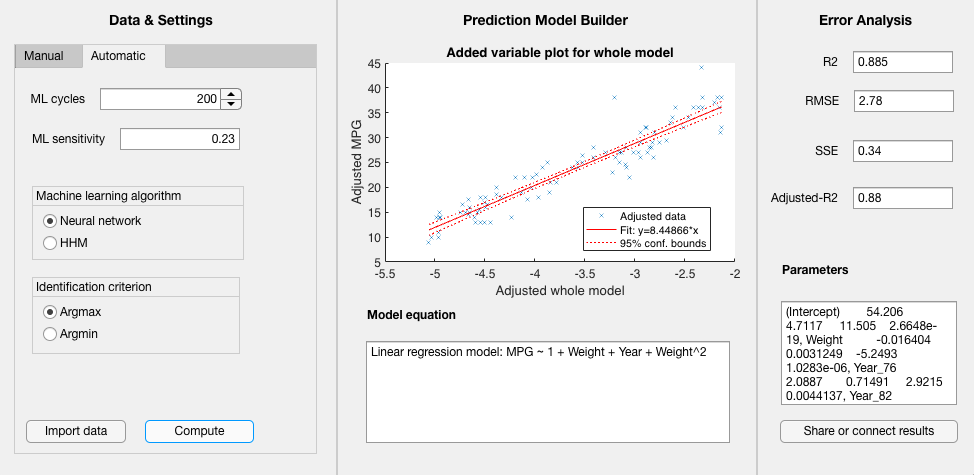
\includegraphics[width=\textwidth]{figures/result.png}
                \caption{Results of prediction}
                \label{fig:results}
            \end{figure}
        \end{center}
        \textbf{Plot of results}\\
        \textbf{Model equation}\\
        \textbf{Parameters}\\